\begin{comment}
\section{Skype}
Skype ist bekannt als Audio- und Videostreaming Lösung, die unter Windows und Linux verwendet werden kann. Es sollte getestet werden, um eine Vergleichsbasis für unsere implementierte Lösung zu haben.
%%%%%%%%%%%%%%%%%%%%%%%%%%%%%%%%%%%%%%%%%%%%%%%%%%%%%%%%%%%%%%%%%%%%%%%%%%
\subsection{Installation}
Konfiguration des Raspian Klienten:
\begin{verbatim}
1.Install and configure PulseAudio.
  sudo apt-get install pulseaudio
  pulseaudio --start
2.set your Raspberry Pi 3 device overclocked in order to achieve good quality
  Skype voice calls. 
  sudo raspi-config
Select Overclock section and then “Pi3” (1000 MHz).
\end{verbatim}

%%%%%%%%%%%%%%%%%%%%%%%%%%%%%%%%%%%%%%%%%%%%%%%%%%%%%%%%%%%%%%%%%%%%%%%%%%
\textbf{Installation ExaGear Desktop}
\begin{verbatim}
3.Laden Sie das ExaGear Desktop-Archiv mit Lizenzschlüssel herunter:
  tar -xvzpf exagear-desktop-rpi3.tar.gz
4.Installieren und aktivieren Sie ExaGear auf Ihrem ARM-Gerät:
  sudo ./install-exagear.sh	 
\end{verbatim}
%%%%%%%%%%%%%%%%%%%%%%%%%%%%%%%%%%%%%%%%%%%%%%%%%%%%%%%%%%%%%%%%%%%%%%%%%%
\subsection{Gast-x86-System}
\begin{verbatim}
5.Geben Sie das Gast-x86-System mit dem folgenden Befehl ein:
 exagear
Starten der Shell im Gastbild /opt/exagear/images/debian-8
Jetzt befinden Sie sich in der x86-Umgebung, die durch Ausführung des Befehls
 'arch' überprüft werden kann:
  arch
  i686
6.aktualisieren apt-get-Repositories beim ersten Start des Gastsystems:
  sudo apt-get update
\end{verbatim}\\

%%%%%%%%%%%%%%%%%%%%%%%%%%%%%%%%%%%%%%%%%%%%%%%%%%%%%%%%%%%%%%%%%%%%%%%%%%
\textbf{Skype vom Raspbian Startmenü ausführen} \\

\begin{minipage}{\textwidth}
    \begin{center}
        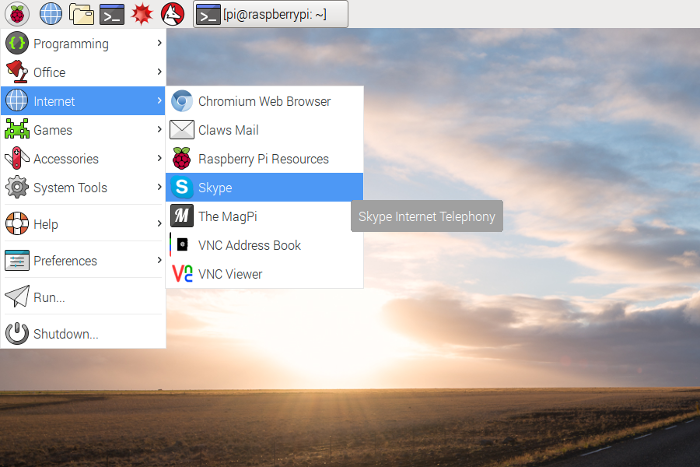
\includegraphics[scale=0.35]{img/skype.png} 
    \end{center}
\end{minipage}
\\

%%%%%%%%%%%%%%%%%%%%%%%%%%%%%%%%%%%%%%%%%%%%%%%%%%%%%%%%%%%%%%%%%%%%%%%%%%
\textbf{Skype Installieren}
\begin{verbatim}
7.Laden Sie Skype für Debian herunter:
  wget http://download.skype.com/linux/skype-debian_4.3.0.37-1_i386.deb
8.Installieren Skype:
  sudo dpkg -i skype-debian_4.3.0.37-1_i386.deb; sudo apt-get install -f
  sudo sed -i 's/4\.3\.0\.37/8\.3\.0\.37/' /usr/bin/skype 
\end{verbatim}
%%%%%%%%%%%%%%%%%%%%%%%%%%%%%%%%%%%%%%%%%%%%%%%%%%%%%%%%%%%%%%%%%%%%%%%%%%
Skype ausführen und überprüfen Sie, ob Skype-Soundgeräte den PulseAudio-Server verwenden:\\

\begin{minipage}{\textwidth}
    \begin{center}        
        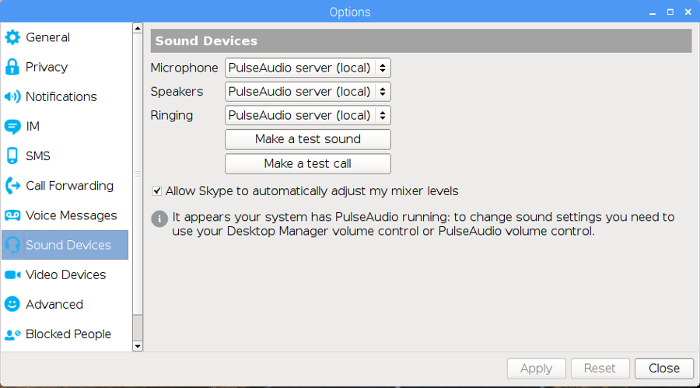
\includegraphics[scale=0.4]{img/skype-option.png} 
    \end{center}
\end{minipage}
\end{comment}
%%%%%%%%%%%%%%%%%%%%%%%%%%%%%%%%%%%%%%%%%%%%%%%%%%%%%%%%%%%%%%%%%%%%%%%%%%
